\documentclass[12pt]{memoir}

\usepackage{titling}

% Figures and controlling packages
\usepackage{float}
\usepackage{wrapfig}
\usepackage{tcolorbox}
\definecolor{coast}{RGB}{255,255,200}

% logo for the title page
\usepackage{adjustbox}
\newcommand{\swlogo}{
  \adjustbox{valign=t}{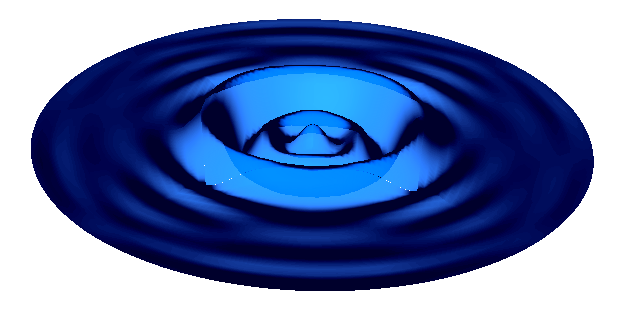
\includegraphics[width=0.25\textwidth]{images/shallowWater.png}}
}

\usepackage{hyperref}
\hypersetup{
    bookmarks=true,         % show bookmarks bar?
    unicode=false,          % non-Latin characters in Acrobat’s bookmarks
    pdftoolbar=true,        % show Acrobat’s toolbar?
    pdfmenubar=true,        % show Acrobat’s menu?
    pdffitwindow=false,     % window fit to page when opened
    pdfstartview={FitH},    % fits the width of the page to the window
    pdftitle={My title},    % title
    pdfauthor={Author},     % author
    pdfsubject={Subject},   % subject of the document
    pdfcreator={Creator},   % creator of the document
    pdfproducer={Producer}, % producer of the document
    pdfkeywords={keyword1, key2, key3}, % list of keywords
    pdfnewwindow=true,      % links in new PDF window
    colorlinks=true,       % false: boxed links; true: colored links
    linkcolor=violet,          % color of internal links (change box color with linkbordercolor)
    citecolor=magenta,        % color of links to bibliography
    filecolor=magenta,      % color of file links
    urlcolor=blue           % color of external links
}
% Adjusting the section,chapter, etc. headings
\usepackage{titlesec}
\newcommand*{\justifyheading}{\raggedleft}

\titleformat{\chapter}[display]
  {\normalfont\sffamily\huge\bfseries\justifyheading\color{blue}}
  {\chaptertitlename\ \thechapter}{20pt}{\Huge}
\titleformat{\section}
  {\normalfont\sffamily\Large\bfseries\color{blue}}
  {\thesection}{1em}{}
\titleformat{\subsection}
  {\normalfont\sffamily\Large\bfseries\color{blue}}
  {\thesection}{1em}{}


\usepackage[margin=1.0in]{geometry}
\usepackage{amsmath,amsthm}
%\usepackage{breqn}
\usepackage{amsfonts}
\usepackage{amssymb}
\usepackage[mathscr]{euscript}
\usepackage{graphicx}
\usepackage{verbatim}
\usepackage[round]{natbib}
\usepackage{appendix}
\usepackage{xcolor}

\linespread{1.5}
% Header and Footer
\makeevenhead{myheadings}{}{}{}
\makeoddhead{myheadings}{}{}{}{}

\makeevenfoot{myheadings}{ {\fontfamily{cmss}\selectfont \theauthor} }{{\fontfamily{cmss}\selectfont \href{mailto:schoonover.numerics@gmail.com}{schoonover.numerics@gmail.com} }}{\thepage}

\makeoddfoot{myheadings}{ {\fontfamily{cmss}\selectfont \theauthor  } }{{\fontfamily{cmss}\selectfont \href{mailto:schoonover.numerics@gmail.com}{schoonover.numerics@gmail.com}} }{\thepage}

\makefootrule{myheadings}{\textwidth}{\normalrulethickness}{0ex}
\chapterstyle{mychapter}
%  Adjust the chapter page footer
\copypagestyle{chapter}{plain}
\makeoddfoot{chapter}{ {\fontfamily{cmss}\selectfont \theauthor  } }{{\fontfamily{cmss}\selectfont \href{mailto:schoonover.numerics@gmail.com}{schoonover.numerics@gmail.com}} }{\thepage}

% Add a line above the footer
\makefootrule{chapter}{\textwidth}{\normalrulethickness}{0ex}

\newcommand{\upperchapterrule}{1.6pt} % upper rule
\newcommand{\lowerchapterrule}{0.8pt} % lower rule
\newcommand{\chapterrulesep}{2pt}     % space between the rules
\newcommand{\chapterruleoffset}{1pt}  % distance of the bottom rule from the baseline

\newcommand{\doublerule}[1]{%
  \vbox{
    \sbox0{ #1 }%
    \dimen0=\textwidth
    \advance\dimen0 by -\wd0
    \divide\dimen0 by 2 % width of the rules
    \noindent
    \makedoublerule
    \usebox{0}%
    \makedoublerule
  }
}

\newcommand{\makedoublerule}{%
  \vbox{
    \hrule width \dimen0 height \upperchapterrule
    \vskip\chapterrulesep
    \hrule height \lowerchapterrule
    \vskip\chapterruleoffset
  }%
}
\author{Joe Schoonover}
\title{}
\date{}




\begin{document}
\frontmatter
% Doing a custom title-page
\begin{titlingpage}
    
        \vspace*{2cm}

   % Setup up the main and sub-titles with the logo
   {\fontfamily{cmss}\selectfont
     \begin{tabular}{l r}
           & \HUGE{\textbf{ Mixed Finite Volume - }}\\
           & \HUGE{\textbf{ Spectral Element Method }}\\
           & \\
           & \huge{\textbf{\textcolor{blue}{Long Topographic Wave}}}\\
           & \huge{\textbf{\textcolor{blue}{ Response Model}}}           
        \end{tabular}
    }    
 
        \vspace{1cm}
        

         
        \vspace{2cm}
        
     \begin{center}
     
        %Do a subtitle here if you like
        {\fontfamily{cmss}\selectfont
        \huge{
           Software Manual
        }
        
        \vspace{1.5cm}
        
        % Enter the author's name
        \textbf{
        \large{
           \theauthor 
         }}}
        
        \vfill
        
        
     \end{center}
        
    
\end{titlingpage}


{\fontfamily{cmss}\selectfont
\tableofcontents
}
\mainmatter

% Special Style
\pagestyle{myheadings}

\chapter{Overview and Motivation}
In studying large scale flows in the ocean, the working equations often used are the Boussinesq and Hydrostatic Primitive equations. These equations filter out explicit statements concerning the cross-geopotential accelerations of fluid parcels and replace the vertical momentum balance with hydrostatic balance. This allows for the pressure to be directly diagnosed from knowledge of the free surface height and the water column density structure. These equations still encompass a large set of complicated dynamics which can be split into gravity waves, in which the pressure signal propagation mechanism is fluid convergences and divergences, and vorticity waves, in which the pressure signal signal propagates due to potential vorticity conservation. When this equation set is placed applied to describing motions in the vicinity of long continental shelves for which the cross-shelf length scale is small in comparison to the along-shelf length scale, scale analysis indicates a favoring of vorticity wave dynamics along the shelf and mixed vorticity-gravity wave dynamics across the shelf. The model developed herein aims to capture both the linear and nonlinear dynamics of this subset of the hydrostatic primitive equations. 


The initial motivation for this formulation is to extend the nonlinear Kelvin wave theory explored by \citet{Dewar_Hogg2010} and \citet{HoggEtAl2011}. A key result from their work illustrated how large scale flows near fluid boundaries can excite small scale motions through the arrest of Kelvin waves. A side effect of this wave arrest is the generation of a counterflow which can lead to flow separation. Given that the ocean sea-floor consists of gradual sloping surfaces (largest slopes are on the order of $10\%$) rather than a flat bottom with vertical side walls, it is reasonable to ask if a similar set of dynamics extends to the more realistic representation of the bottom. Further, can the arrest of topographic waves lead to the separation of oceanic currents, such as the Gulf Stream ? To fully answer these questions, we need to understand (1) the linear response of topographic waves to a large scale flow and (2) the subsequent evolution of unstable linear modes once nonlinear momentum and buoyancy advection become important. The model developed here aims to accomplish these two goals under the filtered set of dynamics of long baroclinic topographic waves.

\section{The equations solved}
Imagine a continental shelf for which the resting fluid depth, the bathymetry, is dominantly described by $z = -h(x)$, where $z$ is the local vertical direction and $x$ is the cross shelf direction. The along shelf direction is denoted by the variable $y$, and we consider motions such that the along shelf length scale, $L_y$, is much larger than the across shelf length scale, $L_x$. Further, we are interested in modelling the topographic wave response to a large scale balanced flow fields interacting with the topography. Because of this, we split the flow field into two parts, (1) a balanced flow which is denoted with an overbar ($\bar{\cdot})$, and (2) an unbalanced flow, denoted with a ``prime'' symbole ($\cdot '$). The final approximation we make is that the topographic response vertical velocity is primarily generated by flow across isobaths which are required to satisfy the no-normal-flow condition. These assumptions lead to a nonlinear elliptic equation in $(x,z)$ for diagnosing the pressure, and a hyperbolic system along the physical boundaries. The elliptic equation for the pressure is an expression of the conservation of potential vorticity. The equations are
\begin{subequations}
\begin{align}
(\bar{p}_{xx} + f^2 + p'_{xx})p'_{zz} + \bar{p}_{zz} p'_{xx} - (2\bar{p}_{xz} + p'_{xz})p'_{xz} &= 0 \\
v'_t + \tilde{u}'(\bar{v}+ v')_s + (\bar{v} + v')v'_y + fu' &= -p'_y \\
b'_t + \tilde{u}'(\bar{b} + b')_s + (\bar{v} + v')b'_y &= 0 \\
\tilde{u}'_s + v'_y &= 0 \\
p'_x &= fv' \\
p'_z &= b'.
\end{align}\label{eq:nonlinearEquations}
\end{subequations}
The coordinate $s$ is the arclength along the physical boundaries. This generalization allows for a vertical wall (as in \citet{HoggEtAl2011}) or for variable bottom topography to be the boundary.  The velocity component $\tilde{u}'$ is the velocity in the $(x,z)$ that is tangent to the boundary everywhere. The variable $u'$ is the zonal velocity and is related to $\tilde{u'}$ via the relationship
\begin{equation}
u' =\tilde{u}' n_z
\end{equation}
where $n_z$ is the vertical component of the boundary unit normal vector $\hat{n} = n_x \hat{x} + n_z \hat{z}$, where $n_x^2  + n_z^2 = 1$.

\textbf{\textit{This point is iterated again, because this seems to cause confusion! $\tilde{u}'$ is the velocity in the $(x,z)$ plane that is tangent to the physical boundary. This means that this equation set is capable of recreating the Kelvin-Wave arrest of \citet{HoggEtAl2011} and naturally generalizes to the variable bottom topography.}}

The linearized equations are
\begin{subequations}
\begin{align}
\left( \bar{p}_{zz} p'_{x} - \bar{p}_{xz}p'_{z}\right)_x + \left( (\bar{p}_{xx} + f^2)p'_{z} - \bar{p}_{xz}p'_{x}\right)_z &= 0 \\
v'_t + \tilde{u}'\bar{v}_s + \bar{v}v'_y + f\tilde{u}' &= -p'_y \\
b'_t + \tilde{u}'\bar{b}_s + \bar{v}b'_y &= 0 \\
\tilde{u}'_s + v'_y &= 0 \\
p'_x &= fv' \\
p'_z &= b'.
\end{align}\label{eq:linearEquations}
\end{subequations}

In either set, the pressure equation can be written as $\nabla \cdot \vec{f} = r$ where $r$ is some residual. In order for a solution to exist, $\vec{f}\cdot\hat{n}$ has to be prescribed on the domain boundaries (where $\hat{n}$ is a unit normal vector) or the pressure must be prescribed. On the topography, the last two conditions of equation set \eqref{eq:nonlinearEquations} (or \eqref{eq:linearEquations}), geostrophy and hydrostatic balance, are used to establish $\vec{f}\cdot\hat{n}$. At the fluid surface, the rigid lid assumption gives $\vec{f}\cdot \hat{n} = 0$. Far from the shelf edge, where there is significant variation in the topography, the pressure anomaly is assumed to decay to zero. So long as the numerical boundary is far enough away, setting the pressure to zero identically at the most offshore boundary suffices. 


\chapter{Solution Algorithm}
Here, the solution algorithm is described in detail which should provide the user with enough information to understand how to setup an experiment with this software. If you are looking to run a black box, a practice that I do not recommend, feel free to skip ahead to the ``QuickStart'' chapter. A basic outline for the solution algorithm over a single time step is summarized in Figure \ref{fig:algorithm}. Here we explain each of the steps in the algorithm.

%\begin{tcolorbox}[colback=coast]
\begin{figure}[h!]
\begin{center}
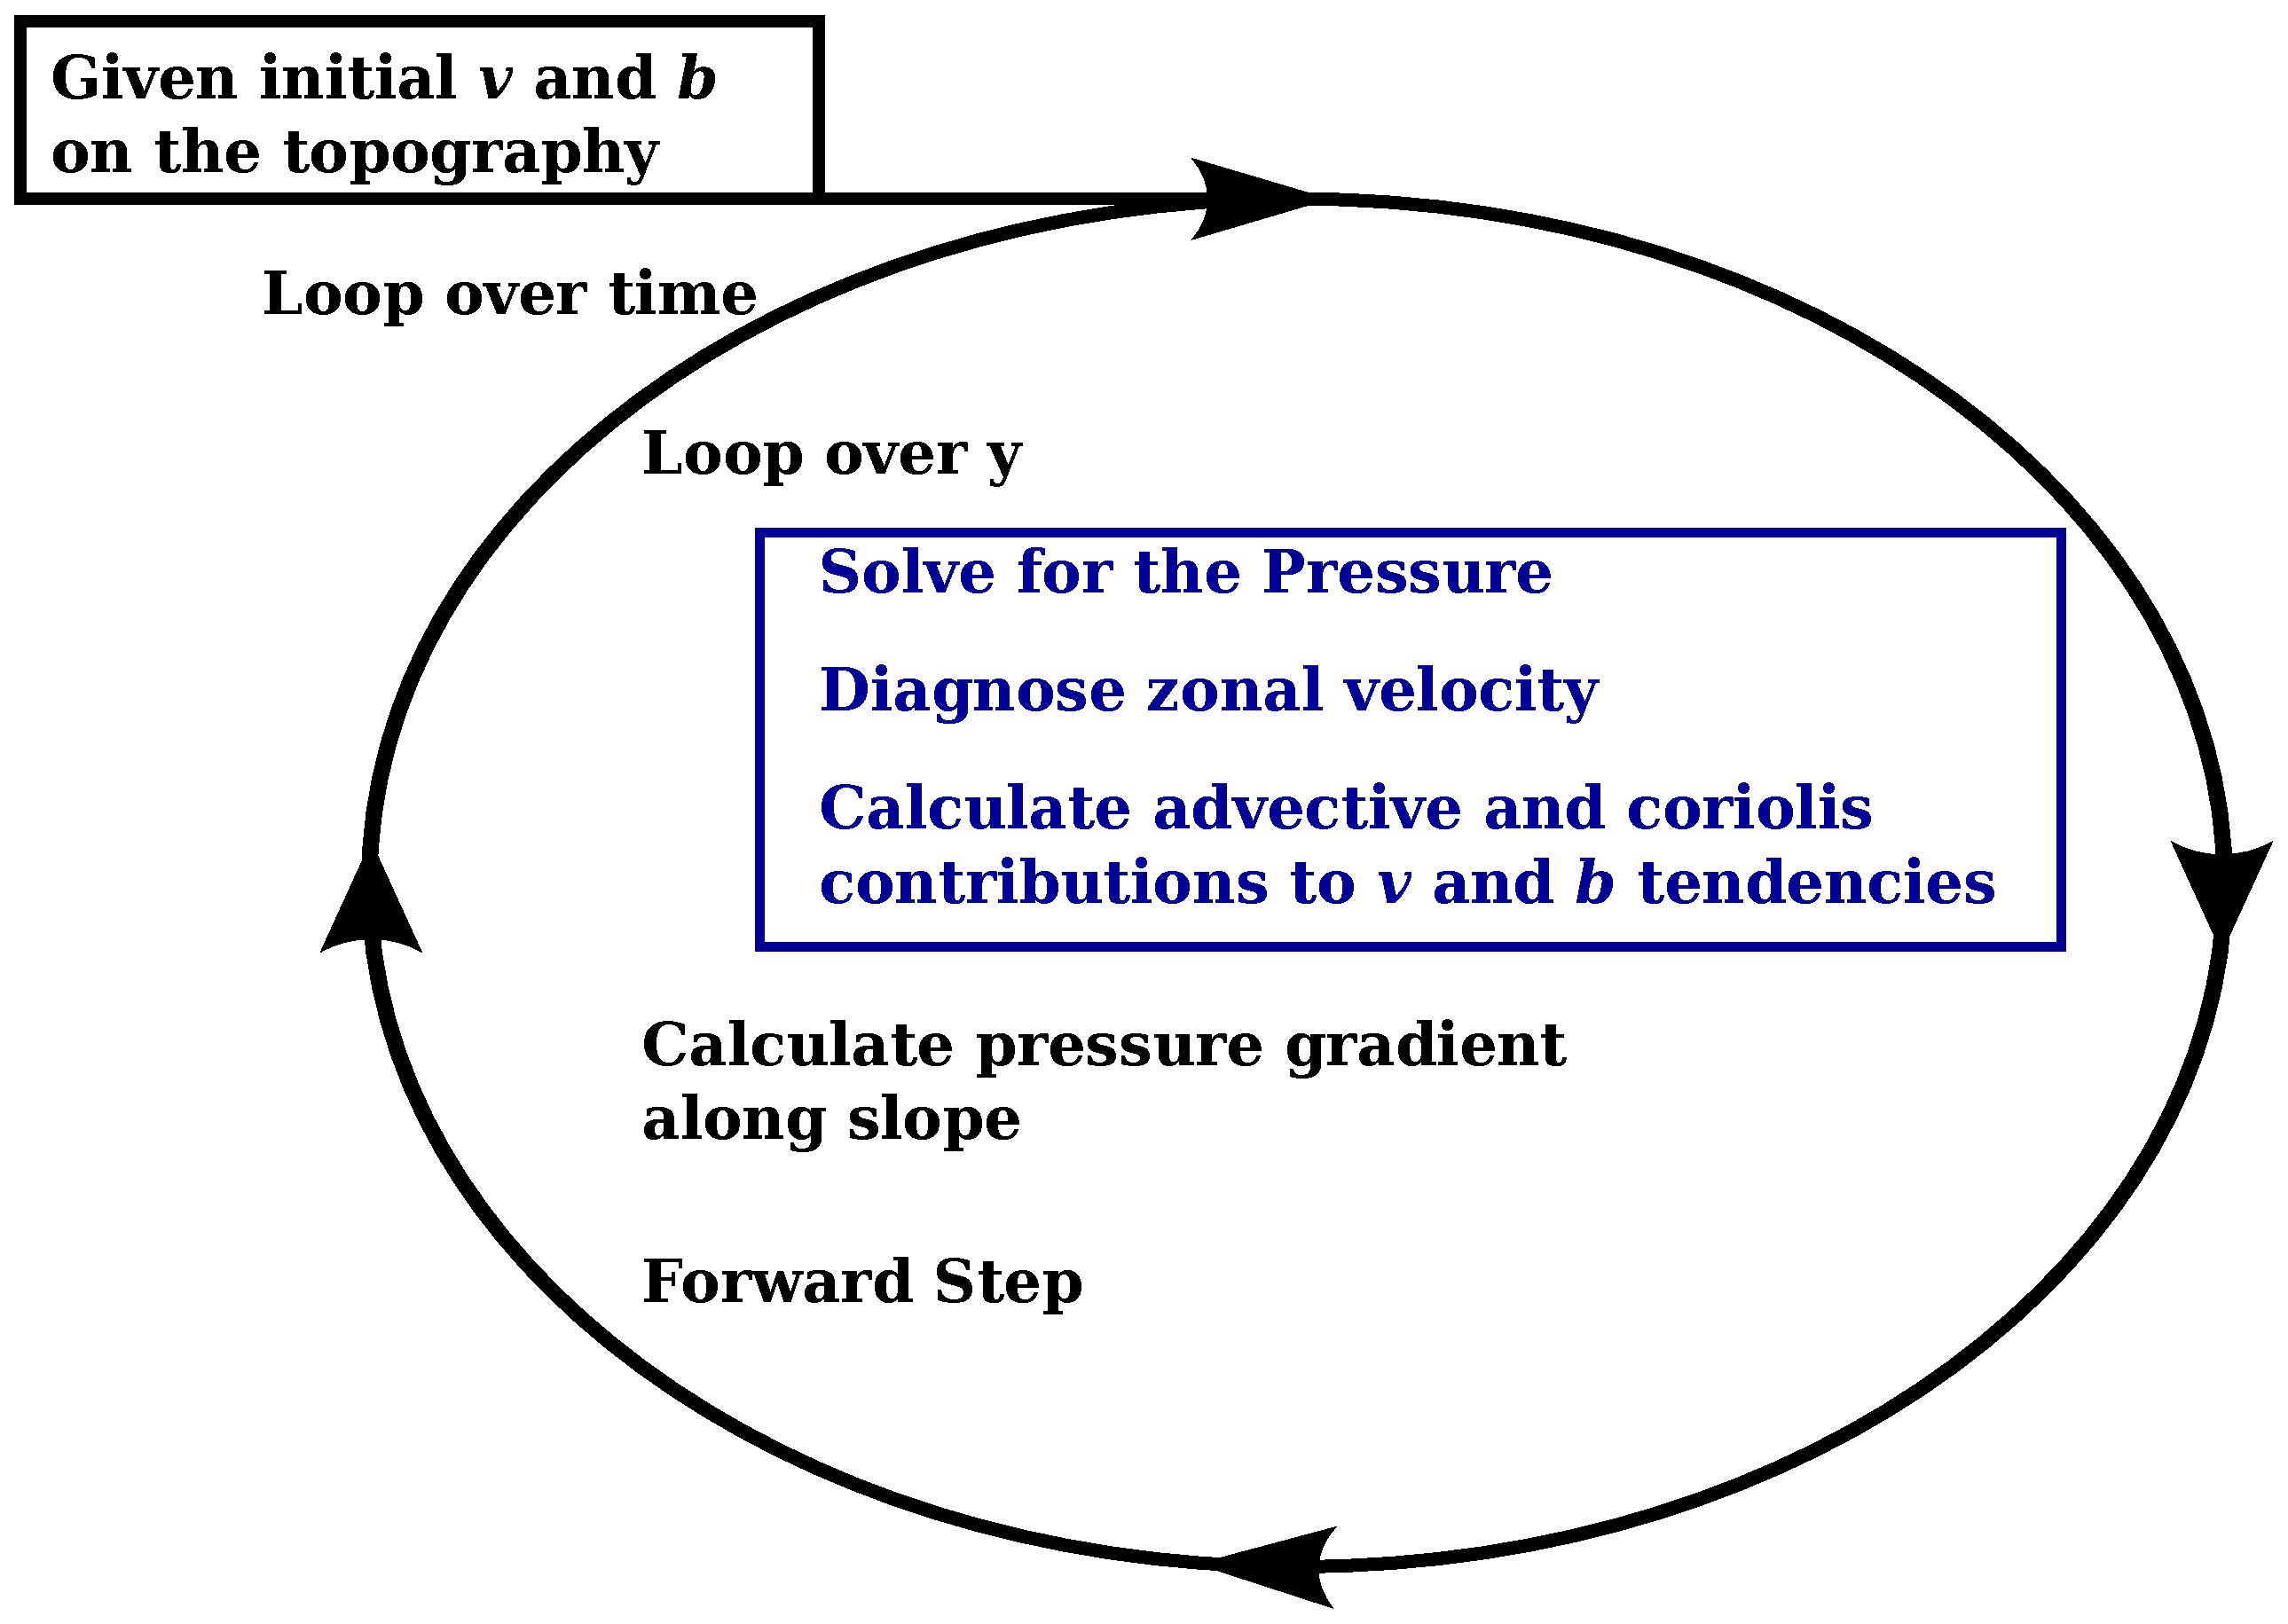
\includegraphics[scale=0.225]{images/topomods/algorithm.eps}
\caption{The diagram above gives a breakdown of the solution algorithm. The textbox in blue indicates the section of the algorithm which uses a spectral element method. The solve for the pressure uses a CGSEM discretization, and the along the topographic slope tendency diagnosis is done with a DGSEM discretization. DGSEM for the latter is chosen due to the hyperbolic nature of the flow along the topographic slope.}\label{fig:algorithm}
\end{center}
\end{figure}
%\end{tcolorbox}

\chapter{QuickStart}


At this point, you have probably unpacked the \texttt{SEM} software libraries in your favorite directory. Here, this will be denoted with ``\texttt{install/dir}.'' This part of the documentation will walk you through the compilation and execution procedures for an instance of the \texttt{DGSEM\_ShallowWater\_Class}. Additionally, steps will be shown for modifying the initial conditions and the mesh to demonstrate the ability to modify the problem. More advanced modifications are discussed in Chapter \ref{chap:Class}. \\

Overall, there are three main steps to performing a simulation
\begin{enumerate}
\item Generate a mesh.
\item Generate initial conditions.
\item Integrate in time.
\end{enumerate}

The first step is achieved by using the SpecMesh software. This generates a mesh from boundary and internal curve inputs in the ``ISM-v2'' format (see the SpecMesh documentation for details on this). Initial conditions are generated using a driver program \texttt{ShallowWater\_Init.f90}. This driver reads in the mesh file output from SpecMesh, computes initial conditions specified by the user within the program, and writes an initial pickup file. Finally, the main driver \texttt{ShallowWater\_Main.f90} reads the mesh and pickup file and performs integration forward in time, manages diagnostic calculations, and file I/O.\\

We will begin by working with the ``gravity-wave'' example. Once you are within the installation directories, you should see the subdirectories
\begin{verbatim}
doc/  examples/  src/  testing/
\end{verbatim}
Change directories into \texttt{examples/} and into the subdirectory \texttt{shallowwater}.
\begin{verbatim}
cd examples/shallowwater
\end{verbatim}
As more validated experiments are conducted with the shallow-water solver, more examples will be found here. For now, we will go into the \texttt{gravity-wave} directory, underneath which you will find the subdirectories
\begin{verbatim}
build/   init/  meshgen/  run/
\end{verbatim}
In the first step, we will modify the make file to ensure we are using the correct compiler and all SEM source directory is set appropriately. The makefile is located in the \texttt{build} directory. Change directories into the \texttt{build} directory and open up the makefile in your favorite text editor. You should see something like 
\begin{verbatim}
# Specify the SEM source code directory
SRCDIR=/home/joe/Desktop/work/SEM/SEM_v2.0/src/
FC=gfortran

# Additional library and includes directories
LIB=
INC= 

# Fortran compilation flags
FFLAGS=-O3 -fopenmp
\end{verbatim}
Set the \texttt{SRCDIR} to the directory where you installed the SEM libraries and include \texttt{src/} at the end (similar to what is shown). Ensure  that the fortran compiler is set appropriately in the variable \texttt{FC}. Lastly, any optimization, debugging, or warning compilation flags should be set under \texttt{FFLAGS}.\\

\chapter{The TOPOGRAPHIC\_RESPONSE Class}\label{chap:Class}

  \section{The Data Structure}

  \section{Routines}
  
  
\pagebreak
\bibliography{references}
\bibliographystyle{plainnat}


\end{document}